\documentclass[tikz,border=0pt]{standalone}
\usepackage[T1]{fontenc}
\usepackage{lmodern,amsmath,amssymb,graphicx,xcolor}
\definecolor{paper}{HTML}{FBF9F5}
\definecolor{ink}{HTML}{172831}
\definecolor{muted}{HTML}{60717A}
\begin{document}
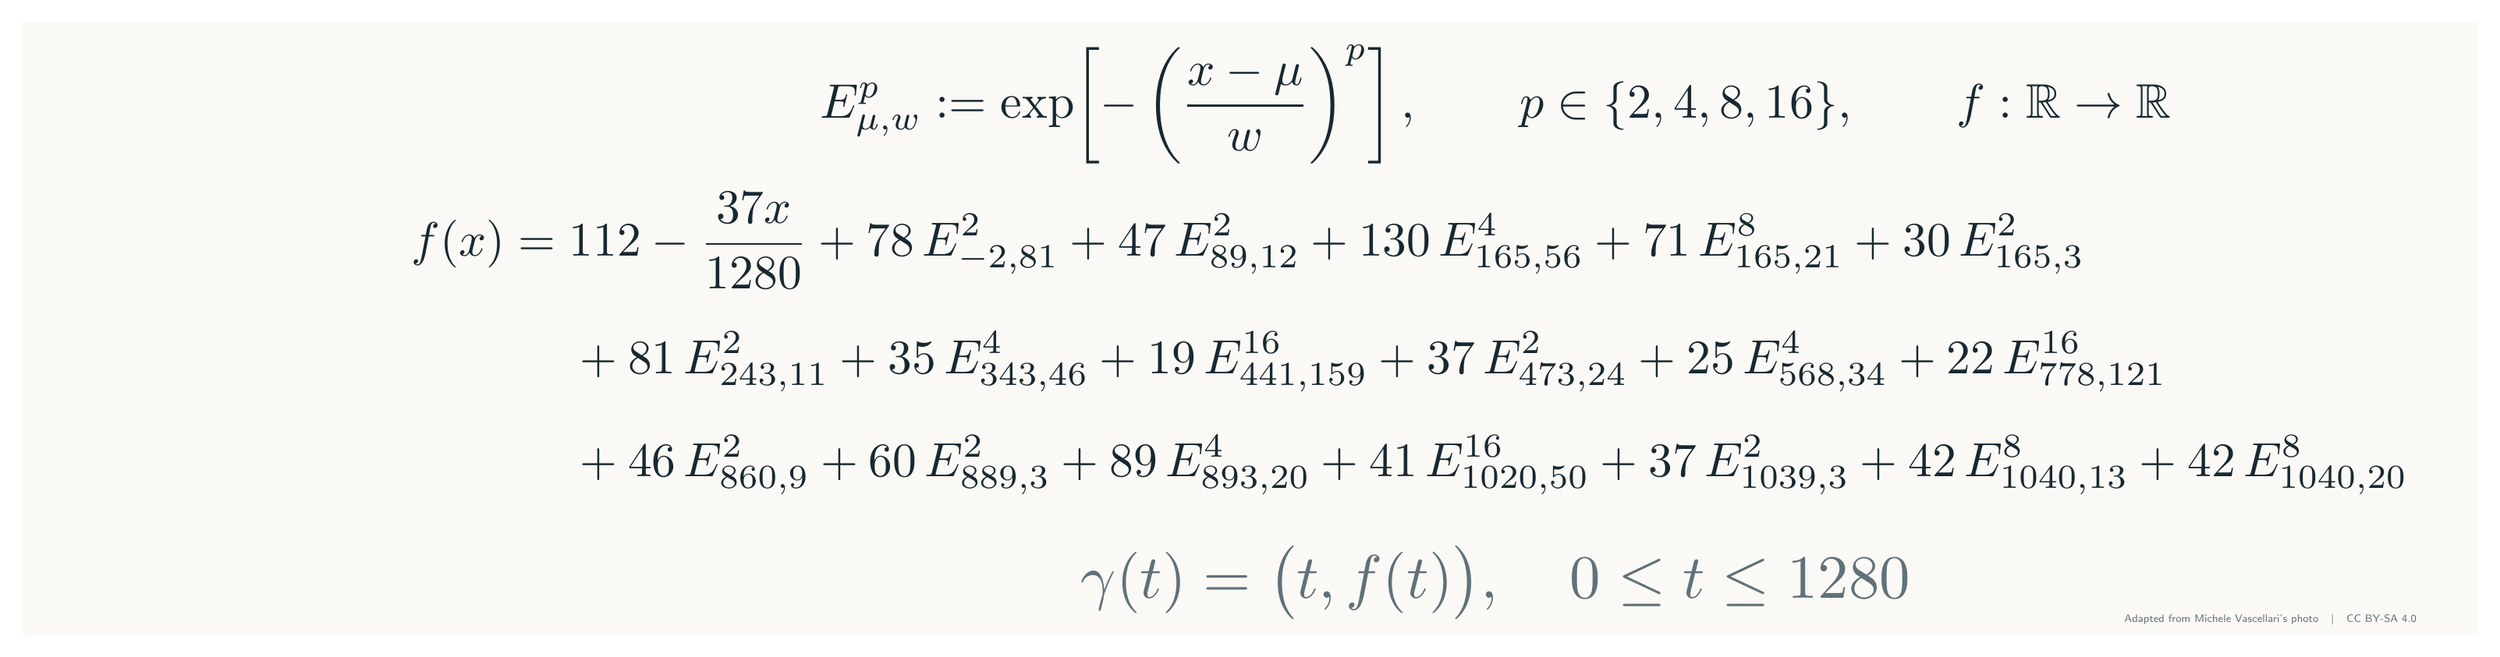
\begin{tikzpicture}[x=1cm,y=1cm,text=ink]
\path[use as bounding box] (0,0) rectangle (40,10);
\begin{pgfinterruptboundingbox}
\fill[paper] (0,0) rectangle (40,10);
\node[inner sep=0pt] at (24,8.65) {\resizebox{22cm}{!}{$\displaystyle
  E^p_{\mu,w}:=\exp\!\left[-\left(\frac{x-\mu}{w}\right)^p\right],
  \qquad p\in\{2,4,8,16\},\qquad f:\mathbb{R}\to\mathbb{R}
$}};
\node[inner sep=0pt] at (22.6,4.75) {\resizebox{32.5cm}{!}{$\displaystyle
  \begin{aligned}
f(x)={}&112-\frac{37x}{1280}+78\,E^{2}_{-2,81}+47\,E^{2}_{89,12}+130\,E^{4}_{165,56}+71\,E^{8}_{165,21}+30\,E^{2}_{165,3}\\[5pt]&+81\,E^{2}_{243,11}+35\,E^{4}_{343,46}+19\,E^{16}_{441,159}+37\,E^{2}_{473,24}+25\,E^{4}_{568,34}+22\,E^{16}_{778,121}\\[5pt]&+46\,E^{2}_{860,9}+60\,E^{2}_{889,3}+89\,E^{4}_{893,20}+41\,E^{16}_{1020,50}+37\,E^{2}_{1039,3}+42\,E^{8}_{1040,13}+42\,E^{8}_{1040,20}
  \end{aligned}
$}};
\node[inner sep=0pt,text=muted] at (24,0.85) {\resizebox{13.5cm}{!}{$\displaystyle
  \gamma(t)=\bigl(t,f(t)\bigr),\quad 0\leq t\leq1280
$}};
\node[anchor=east,inner sep=0pt,text=muted] at (39,0.25)
  {\fontsize{5.3}{6}\selectfont\sffamily Adapted from Michele Vascellari's photo\quad\textbar\quad CC BY-SA 4.0};
\end{pgfinterruptboundingbox}
\end{tikzpicture}
\end{document}
